\documentclass[a4paper]{article}
\usepackage{ctex}
\usepackage{xeCJK}
\usepackage{amsmath}
\usepackage{amsfonts}
\usepackage{amssymb}
\usepackage{graphicx}
\usepackage{colortbl}
\usepackage{fancyvrb}
\usepackage{longtable}
\usepackage{xcolor}
\usepackage[hidelinks]{hyperref}
\usepackage[affil-it]{authblk}
\usepackage[top = 1.0in, bottom = 1.0in, left = 1.0in, right = 1.0in]{geometry}
\usepackage{amsthm}

\setCJKfamilyfont{kai}{KaiTi_GB2312}
\newcommand{\kai}{\CJKfamily{kai}}

\setCJKfamilyfont{song}{SimSun}
\newcommand{\song}{\CJKfamily{song}}

\newcommand\spc{\vspace{6pt}}
\newcommand{\floor}[1]{\lfloor {#1} \rfloor}
\newcommand{\ceil}[1]{\lceil {#1} \rceil}
\newcommand*\chem[1]{\ensuremath{\mathrm{#1}}}

\newtheorem{theorem}{Theorem}[section]
\newtheorem{lemma}[theorem]{Lemma}
\newtheorem{problem}{例题}

\date{\today}
%\date{\yestoday}
\title{网络流总结}
\author{$\mathcal Idvz$}

\begin{document}

\maketitle

%\kai

\song

\tableofcontents

\newpage

\section{\kai{最大流模型}}

最大流的模型一般为每一条从源点到汇点的路径都对应着一种方案,而要求最大化某种值。

同时,最大流也可以适用与二分图,例如求最大匹配等等。

最大流与费用流的结合放到后面讲。

从几个经典问题入手。

\subsection{\kai{简单最大流模型}}

\begin{problem}
  第一题%\footnote{bzoj2957}

  给出$n\times m(n \le m)$的矩阵D,在满足选出的$n$个数不在同行或者同列下第$k$大的数字的最小值。
  
  数据范围:$1\le k\le n\le m\le 250$
\end{problem}

首先我们知道,要求第$k$大的数字最小,这个可以通过$log$的时间复杂度转化成判定性问题。

问题要求满足选出的数不在同一行或列,这个限制是可以转化成二分图的模型,即将行作为二分图的$A$部点,列作为二分图的$B$部点。

考虑只能选择一次,我们可以通过限流达到目的,$s$连接$A$部点,$B$部点连到$t$,容量均为$1$,同时将$D_{i,j}$所在的行$i$连到列$j$,容量为$1$。

观察建出来的图,$s-i-j-t$恰好对应这选择数字$D_{i,j}$的方案,同时流量限制每行列只能被选择一次。

每次二分答案$g$,将所有小于等于$g$的数加入到图中,判断跑出来的最大流是否大于等于$n-k+1$即可。

{
\kai

  考虑证明二分答案的正确性,对于二分的最后结果$ans$,显然是有$n-k+1$个数小于等于$ans$,而没有$n-k+1$个数小于等于$ans-1$,那么至少会有$k$个数大于等于$ans$。

  既有$n-k+1$个数小于等于$ans$,又至少有$k$个数大于等于$ans$,即$ans$为第$k$大的数字。
  
}

~\\
~\\


\begin{problem}
  第二题%\footnote{ZJOI2007}

  给出$n$个点$m$条边的有向无环图,现在有$k$个人从$1$号点出发到达$n$号点,要求每个人每时刻都必须沿着一条边走,不能不走(除非到达点$n$),同时每条边每个时刻只能有一个人经过。

  询问最晚到达点$n$的人的最早时间。

  数据范围:$n\leq 100, m,k\leq 10^3$
\end{problem}

最晚到达点$n$的人的最早时间,继续二分,我们可以通过时间构造分层图,再通过最大流对应方案达到限制。

这里的每一条边在每一天中都只能经过一次,自然地流量为$1$,每个人都必须选择一条边走,所以我们把当前时间的图中的点连到下一天的图中能够到达的点。

\newpage

\begin{problem}
  第三题

  给出$n\times m$的棋盘,其中某些格子是障碍,要求在棋盘上放棋子。

  对于每行给出非负整数$l_i$,表示每行至少放置$l_i$个,每列给出$c_i$,表示至少放置$c_i$个。

  要求放置最少的棋子满足要求。
  
  数据范围:$n,m\leq 100$
\end{problem}

正着做比较麻烦(\sout{不表示不能做}),题目要求放置最少,我们假设一开始所有格子全部放置棋子(除去障碍点),问题转化成了删去最多的棋子使其满足要求。

依旧将行与列看作二分图的$AB$部,源点向$A$部连接容量为每行能够删去的棋子个数,$B$部向汇点连接容量为每列能够删去的棋子个数,中间再将能够删去的棋子的行与列连接。

依旧是最大流对应方案问题。

\newpage

\section{\kai {最小割模型}}

此处略去关于最小割定义。

\subsection{\kai 从最小割定义出发的构图}

\begin{problem}
  第四题

  给出一张$n$点$m$边的无向图,每条边的边权为$D_i$。

  你可以进行一种操作,即将除了某边之外的所有边的权值减少$1$。

  求使得某条边一定在最小生成树中的最少操作次数。

  数据范围:$1\le n\le 500,1\le m\le 800,1\le D_i\le 10^6$
  
\end{problem}

回忆一下$kruskal$算法求最小生成树的步骤,如果$(u,v,w)$这条边一定在最小生成树中,那么边权小于$w$的所有边都不能使得$u,v$联通,\sout{显然的最小割}。

考虑操作,该操作等价于将该边的权值加上$1$,所以我们只需要考虑在原图中所有小于$w$的边,用最小的代价让$u,v$不联通。

经典的从定义出发的构图模型。

\subsection{\kai{最小割与最大权闭合子图}}

一般模型为选择某个收益的前提是选择其他的收益,对于有前提条件的选择基本可以转化到这个模型上。

来看一道特别明显的题。

\begin{problem}
  第五题%\footnote{Heoi2013 day1}

  给出两棵$n$个节点的无根树(不保证同构),每个点有权值$w_i$。

  现在要求选出一些节点,使得选出的节点在两棵树中都能构成联通子图。

  求合法方法中的最大的$\sum\limits_{i\in subset}w_i$

  数据范围:$1\le n\le 50$

\end{problem}

由于$n$非常的小,同时这是两个无根树,联通子图并没有根,但是我们可以通过枚举根来寻找最优值,接着所有节点的父子节点已经确定了。

继续观察问题,由于是联通子图,于是变成了选择儿子节点的前提必须选择父亲节点。

剩下的就是明显的最大权闭合子图问题啦

\newpage

\subsection{\kai{最小割与二元组模型}}

这是一种玄妙的姿势,通过建立最基本的二元关系来建图。

常见模型为两件物品,同时选或者不选将会获得不同的额外收益,这样的模型都可以通过转化为二元组模型解决。

从最基本的问题入手。

\begin{problem}
  第六题

  给出$n\times m$个人,每个人划分到$A,B$集合的收益分别为$a_{i,j},b_{i,j}$。

  同时若相邻人(仅$1$人)与自己同时划分到$A$或$B$集合将会获得额外收益$s_{i,j},r_{i,j}$。

  求获得的最大收益。

  数据范围:$1\le n,m\le 100$
  
\end{problem}

来看一张经典的二元组模型的图。

\begin{figure}[htb]        
    \center{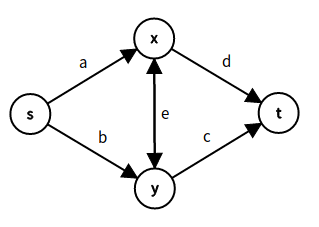
\includegraphics[width=5cm]  {graph1.png}}        
\end{figure}

由于我的思维习惯考虑划分到某集合后的损失,所以下面讨论的所有模型均只考虑损失。

$x,y$表示两个待选择的人,$s$表示$A$集合,$t$表示$B$集合,我们考虑列出方程组。

这里暂时不考虑每个人单独的损失。

\begin{eqnarray} 
  a+b &=& s_{x,y} \\
  c+d &=& r_{x,y} \\
  a+e+c &=& s_{x,y}+r_{x,y}\\
  b+e+d &=& s_{x,y}+r_{x,y}
\end{eqnarray}

$(4)+(3)-(2)-(1)$,解方程得到:

\begin{eqnarray*} 
  a = b &=& \frac{s_{x,y}}{2} \\
  c = d &=& \frac{r_{x,y}}{2} \\
  e &=& \frac{s_{x,y}+r_{x,y}}{2} 
\end{eqnarray*}

考虑同时乘上$2$得到

\begin{eqnarray*} 
  a = b &=& s_{x,y} \\
  c = d &=& r_{x,y} \\
  e &=& s_{x,y}+r_{x,y} 
\end{eqnarray*}

由于做了乘法,在最后处理答案的时候需要逆处理。

考虑每个人的选择收益,由于需要除以$2$,而本身并没有出现在上述的讨论中,所以需要在建边的时候将边权乘上$2$。

所以答案为$$\sum_{i,j}(a_{i,j}+b_{i,j}+s_{i,j}+r_{i,j}) -\frac{minimalcut}{2}$$

~\\
~\\

继续看一道不是那么经典的模型。

~\\

\begin{problem}
  第七题

  给出$n\times m$的矩阵,对于第$i$行$j$列的格子,若划分到$A$集合将获得收益$A_{i,j}$,若划分到$B$集合,将获得收益$B_{i,j}$。对于四联通的格子,若存在$k(0\le k \le 4)$个格子与$(i,j)$所在的集合不同将获得$k\times C_{i,j}$的收益。

  求最大收益。

  数据范围:$1\le n,m\le 100$
\end{problem}

观察一下,这道题与上一道题的不同之处在于这一题的划分在不同集合将会获得额外收益。

若继续按照上面的方式建立方程将会导致问题:解得的$e\le 0$,这样将无法套用二元组的模型。

\begin{figure}[htb]        
    \center{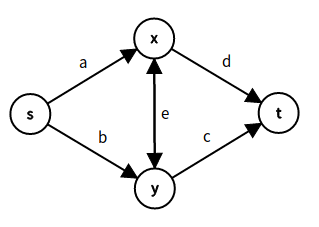
\includegraphics[width=5cm]  {graph1.png}}        
\end{figure}

但是是可以解决的,我们重新规定一下。

对于$x$而言,$s$表示$A$集合,$t$表示$B$集合,对于$y$而言,$s$表示$B$集合,$t$表示$A$集合。

特别地,这里的额外收益是互相的。

这样我们可以重新列出方程组

\begin{eqnarray} 
  a + b &=& A_x+B_y \\
  c + d &=& B_x+A_y \\
  a+e+c &=& A_x+A_y+C_{x,y}+C_{y,x}\\
  b+e+d &=& B_x+B_y+C_{x,y}+C_{y,x} 
\end{eqnarray}

\newpage

按照套路处理方程得到

\begin{eqnarray*} 
  a &=& A_x \\
  b &=& B_y \\
  c &=& B_x \\
  d &=& A_y \\
  e &=& C_{x,y}+C_{y,x}
\end{eqnarray*}

到这里已经处理完全了,回到原问题,我们强行将$y$的边反向,这样在某些情况下会出现矛盾,即非二分图中,我们并不能确定$y$是否该反向。

所以在此之前,我们应该将矩阵做黑白染色。

~\\
~\\

不是明显的二元组模型,我们也可以通过转化变成二元组模型。

\begin{problem}
  第八题

  给出$n\times m$的矩阵,若$(i,j)$划分到$A$集合获得收益$A_{i,j}$,划分到$B$集合获得收益$S_{i,j}$。

  同时对于$(i,j)$,若四联通的格子与$(i,j)$均划分到$A$集合,将会获得收益$sa_{i,j}$,若同时划分到$B$集合,将会获得收益$sb_{i,j}$。

  求最大收益。

  数据范围:$1\le n,m\le 100$
\end{problem}

与四个格子划分到同一集合,看上去并不是二元组模型,但是可以转化为二元组问题。

我们新增加两个节点分别表示周围四个格子同时选择$A,B$集合。

还是原来的那张图?

\begin{figure}[htb]        
  \center{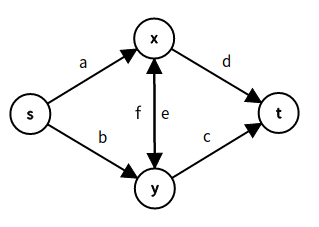
\includegraphics[width=5cm]  {graph2.png}}        
\end{figure}

依旧需要重新规定一下。

$f$表示边$(x,y)$的边权,$e$表示$(y,x)$的边权,$x$表示某个格子,$y$表示周围格子同时划分到$A$集合。

\newpage

不再是原来的方程?

\begin{eqnarray} 
  a + b &=& A_x+sa \\
  c + d &=& B_x \\
  a + e + c &=& A_x + inf \\
  b + f + d &=& B_x + sa 
\end{eqnarray}

对于$(11)$中,在实际问题中并不会出现这种情况,所以需要强制设置为$inf$。

继续解方程。

\begin{eqnarray*} 
  a &=& A_x \\
  b &=& sa \\
  c &=& 0 \\
  d &=& B_x \\
  e &=& inf \\
  f &=& 0
\end{eqnarray*}

对于边权为$0$的边,我们在建边的时候忽略这条边。

对于同时划分到$B$集合的收益,只需要重复上面的步骤即可,在此不再赘述。

\sout{(是不是和意识流的建边一模一样?)}

\subsection{\kai{最小割与距离限制模型}}

权值线段树即按权值建树,适用于一些不要求询问区间的题目(充当普通平衡树的作用),或者是通过树套树或线段树合并乃至可持久化来支持询问一些特殊的东西。

充当普通平衡树,其实就是把元素的权值当作下标插入到线段树中,然后利用线段树来维护这些元素的一些性质。

因为这个很水所以我就不举例子了。

\section{\kai{可持久化线段树的基础应用}}

如果两棵线段树之间有许多相同的节点可以共用,那么我们可以考虑用可持久化线段树让它们共用节点。

可持久化线段树最基本的应用就是通过区间的差分来维护给定区间的一些信息,当然也可以用树套树……。

\subsection{\kai{一类维护序列中某个区间信息的问题}}

\begin{problem}
  网络管理\footnote{CTSC2008}

  给出一棵$n$个点的树,每个点有一个值$w_i$。有$m$个操作。

  1.给出$a,b$,将$w_a$变成$b$。

  2.给出$a,b,k$,询问从$a$到$b$的路径中第$k$大的值。

  数据范围:$n,m\leq 80000, w_i\leq 10^8$。
\end{problem}

这是一个经典问题。

我们对于每个节点开一棵权值线段树,维护从根节点到自己的所有$w$。

因为每个节点相对于父亲节点只是插入了一个$w$,所以可以用可持久化线段树,每次插入复杂度为$O(\log n)$。

那么询问的话就是两个端点的权值线段树减去LCA的权值线段树(注意细节即可)。

修改一个点的值只会影响它的子树。

于是我们按照dfs序建树状数组,树状数组的每个节点维护一棵权值线段树。

修改点值就相当于在它的子树这一段连续的dfs序区间中每个点修改值,用树状数组的区间修改、单点查询的方法就能够在 $O(n\log n^2)$ 的时间内解决本题。

\sout{这就是伟大的树上带修改第k大。}

\bigskip

这类问题满足的性质就是维护的信息满足可加减性,然后就可以用可持久化线段树来动态维护信息了。

\begin{problem}
  k seq\footnote{hihocoder 1046}

  给出一个长度为$n$的序列$A$和$k$。

  定义一个子串的$w$为子串中,相同的数字只计算一次,所有的数的和。

  求第$k$大的$w$。

  数据范围:$n, k\leq 10^5$
\end{problem}

因为一个子串总能被表示成一个后缀的前缀,所以我们对于每个位置$i$维护一个普通线段树$S[i]$,里面下标为$j$的元素是$w[i..j]$的值。同时维护一个最大值。

首先我们先暴力预处理出普通线段树$S[1]$。

然后往后枚举每一个位置,对于每一个位置$i$,记上一个位置的那个元素下一次出现的位置为$pos$。

则对于$j\in [i, pos - 1]$,$S[i]$中下标为$j$的元素的值就等于$S[i-1]$中下标为$j$的元素的值减去$val[i-1]$,其他下标的元素的值不变。

使用可持久化线段树,使用懒标记,于是每个位置只需要花费$O(\log n)$的时间就可以构造出线段树。

我们把每个位置的线段树的最大值放到一个堆里面。

每次找出最大的那个位置,然后将最大的那个后缀的最大的那个前缀的位置上的值改成无穷小,求出最大值之后再次插入堆中。

这个操作重复$k$次即找出第$k$大值。

复杂度为$O((n+k)\log n)$。

\section{\kai{动态开点线段树的基础应用}}

一般动态开点线段树的应用情况就是要开的节点太多,但是实际用到的节点特少的情况下,我们可以用指针树的方法动态开线段树的节点。

动态开点线段树的应用很广泛,可持久化线段树若有若无地用到了这个思想,线段树合并则是这个东西的具体应用。

下面我给出一道体现“开点开不下”的例题。

\begin{problem}
  旅行\footnote{Sdoi 2014}

  给出一棵$n$个点的树, $q$个操作。每个点有两个值。

  1.给出$x,c$,将第$x$个点的第一个值改成$c$。

  2.给出$x,c$,将第$x$个点的第二个值改成$c$。

  3.给出$x,y$,询问第$x$个点到第$y$个点经过的路径中,第一个值与$x$的第一个值相同的点,第二个值的和。

  4.给出$x,y$,询问第$x$个点到第$y$个点经过的路径中,第一个值与$x$的第一个值相同的点,第二个值的最大值。

  数据范围:$n,q\leq 10^5, c\leq 10^5$
\end{problem}

好吧这就是一个水题,我们对于每个“第二个值”开一棵线段树,即$10^5$棵线段树维护每个位置,然后用树链剖分即可。

因为每棵线段树的极限空间是$O(n)$的,所以空间复杂度是$O(nc)$的。

但是因为总的节点数量不超过$O(n)$,所以动态开点即可,空间复杂度为$O(n)$。

下面应该还有一些要用到动态开点的题目。

\section{\kai{线段树合并的基础应用}}

线段树合并就是动态开点的线段树合并在一起,使用条件是总点数为$O(n)$,则复杂度为$O(n\log n)$。

具体实现方法就是哪里有点就往哪里合并。

\subsection{\kai{一类考虑子树对父亲的贡献的问题}}

这种题目看起来就像树形dp,就是从每个点维护一棵线段树,然后合并到父亲那里去。

\begin{problem}
  天天爱跑步\footnote{noip2016}

  给出一棵$n$个节点的树,$m$条有向路径,每个节点有一个值$v_i$。

  对于每个节点,询问有多少条经过它的有向路径,且它到这条路径的起点的距离为$v_i$。
\end{problem}

这个题我学习了一下线段树合并的做法。

对于一条有向路径,将它的信息记录在两个端点上,因为路径上的其它点一定是两个端点其中一个的父亲,于是可以用树形dp的思想。

对于这条路径的信息,我们经过左右端点的时候记录在线段树中,在经过它们的LCA的父亲的时候删除。

经过每个点,我们在线段树中查找,是否有一条路径走到它的时候距离为$v_i$。

这个查询需要用到下文中“下标有关”的思想,其实也很容易,将距离与自己的深度拆开即可。

于是经过一个节点,首先合并子树,然后删除信息,最后进行查询。

复杂度为$O(n\log n)$。

\bigskip

下面是一个更加容易看出这种思想的题目。

\begin{problem}
  Tree Rotations\footnote{Poi2011}

  现在有一棵二叉树,所有非叶子节点都有两个孩子。在每个叶子节点上有一个权值(有$n$个叶子节点,满足这些权值为$1..n$的一个排列)。

  可以任意交换每个非叶子节点的左右孩子。
  
  要求进行一系列交换,使得最终所有叶子节点的权值按照遍历序写出来,逆序对个数最少。
\end{problem}

首先对于每个节点维护一个权值线段树。

因为对于一个节点交换其左右子树对于左右子树中自己的逆序对没有影响,所以我们可以用类似树形dp的方法。

一个节点的逆序对数量等于左右子树中最少的逆序对数量,加上是否交换左右子树产生的跨树的逆序对的数量。

这个跨树的逆序对我们只需要在合并左右两颗权值线段树的时候顺带统计一下就好了。

于是可以在$O(n\log n)$的时间内解决此题。

\bigskip

下面是一个另一种风格的题目。

\begin{problem}
  安全路径\footnote{Usaco Jan09}

  给出一张点数为$n$,边数为$m$的无向图,对于每个点,询问从第一个点到这个点的,不经过最短路的最后一条边的最短路的长度。

  保证对于每个点只有一条最短路。

  数据范围:$n\leq 10^5,m\leq 2\times 10^5$
\end{problem}

首先构出最短路径树,因为不经过最后一条边,所以删掉这条边之后,第一个点到这个点在最短路径树上不连通。

那么只能从这个点的子树中的某个点往上走到这个点。

对于它(编号为$j$)的子树中的一个点$i$,和这个点的一条进来的非树边的起点$e$,贡献是$dis[1][e]+dis[e][i]+depth[i]-depth[j]$

于是我们把子树中的所有点以及它们的非树边的$dis[1][e]+dis[e][i]+depth[i]$放到权值线段树中。

则一个点的答案就是权值线段树中的最小值减去$depth[j]$的值。

我们一路线段树合并上去就能在$O(n\log n)$的时间内解决此题。

\section{\kai{线段树套线段树的基础应用}}

线段树套线段树其实就是在线段树的每个节点都开一棵线段树。

这种题目也是烂大街了,可持久化线段树的题目一般都能改成树套树,复杂度不变或增大几个$log$。

这里举一个特殊一点的树套树的题目的例子。

\begin{problem}
  K大数查询\footnote{Zjoi 2013}

  有$n$个位置,$m$个操作。操作有两种,每次操作如果是$1\ a\ b\ c$的形式表示在第$a$个位置到第$b$个位置,每个位置加入一个数$c$

  如果是$2\ a\ b\ c$形式,表示询问从第$a$个位置到第$b$个位置,第$C$大的数是多少。

  数据范围:$n,m\leq 50000$
\end{problem}

这个题目如果想要每个位置分别维护元素的话显然元素个数要爆炸。

所以我们考虑怎么每个元素分别维护。

于是我们用树套树,权值线段树套位置线段树,即每一个权值我们开一棵线段树,表示哪些区间中有这个权值。

询问的时候从权值线段树自上往下走,查询个数的时候深入到位置线段树中即可。

时间复杂度为$O(n\log^2 n)$

\section{\kai{线段树作为辅助数据结构的一些问题}}

除了裸的数据结构题之外,还有一些题目线段树是作为辅助数据结构来使用的,主体算法往往不是线段树。

\subsection{\kai{用线段树优化dp}}

这个是老生长谈了。

我就举一道考试题作为例子吧。

\begin{problem}
  永远亭的竹笋采摘\footnote{test20170331}

  辉夜原本是生活在月宫的月之公主。

  在永远亭中,有一排新鲜的$n$个竹笋。辉夜对他们很是喜欢,于是决定采摘一些来制作$k$份料理。她找出了一个曾经在月都使用过的工具,凑合凑合可能可以用来采摘竹笋。这个工具每次可以采摘连续的一段竹笋,并用这些竹笋自动做出一份料理。但为了避免对工具造成损坏,这连续的一段中的竹笋必须都是未经过采摘的。辉夜依次给每颗竹笋标注了卡路里$a_0, \ldots, a_{n - 1}$,拥有很棒很棒很棒身材的她当然不想摄入过多的能量。用竹笋制作出的料理的能量是所有选出的竹笋中卡路里相差最小的两个卡路里不同的竹笋。每次采摘的竹笋中至少要有2个卡路里不相同的笋子。

  辉夜想知道,她使用工具采摘竹笋能够获得的最少能量是多少。

  $1 \leq n \leq 50000, k \leq 1000, k \leq n/2$,保证数据可以制作$k$份料理。$a_i$的值均是正整数且不超过$n$。
\end{problem}

萌萌的DP题。

那么不妨设$f_{i, j}$表示在$1..j$的范围内使用了$i$个区间的最小答案。不难写出转移方程:
$$f_{i, j} = \min\{f_{i, j - 1}, f_{i - 1, k} + g(k, j)\}$$

其中$g(k,j)$代表区间$k..j$中最小的两个不同的数的差。

那么不难得到$g(k,j)$的转移方程:
$$g(k,j) = min(|a_k - a_j|, g(k+1,j), g(k,j-1)) | a_k \neq a_j$$

不难发现,这样DP是做了冗余操作的,即假设$k..j$之间差最小的是$|a_x - a_y|$,那么对于那些$k \leq p < x$或$y < p \leq j$的点,他们既可以被选入这个区间,又可以不被选入,也就是答案相同的区间我们进行了$(x-k)\times(j-y)$次枚举,实际上只有1次是有意义的。

那么我们把两个DP写在一起:
$$f_{i, j} = \min\{f_{i, j - 1}, f_{i - 1, k} + |a_j - a_k|\} | a_j \neq a_k$$

终于有个靠谱一点的方程了,考虑优化。

把绝对值拆开,把$a_j$提到$\min$外面,可得:
\begin{displaymath}
  f_{i, j} = \left\{ \begin{array}{ll}
    \min\{f_{i, j - 1}, f_{i - 1, k} - a_k\} + a_j & a_j > a_k \\
    \min\{f_{i, j - 1}, f_{i - 1, k} + a_k\} - a_j & a_j < a_k
  \end{array} \right.
\end{displaymath}

至此我们可以用线段树优化至$O(nk\log n)$,即将DP值以$a_i$为关键字记录在线段树里面即可,但这个算法常数较大。

\subsection{\kai{用线段树判断完美匹配}}

一些特殊的完美匹配问题可以用线段树来解决。

\begin{problem}
  lyz\footnote{POI2009}

  滑冰俱乐部初始有$1..n$号码溜冰鞋各$k$双,已知$x$号脚的人可以穿$x..x+d$号码的鞋子。现在有$m$次操作,每次两个数$r$、$x$,表示$r$号脚的人来了$x$个,$x$为负表示离开。对于每次操作,输出溜冰鞋是否足够。

  数据范围:$n,k,m\leq 5\times 10^5, k\leq 10^9$
\end{problem}

我们把人看作一个点集,溜冰鞋看作另一个点集,则题目转化为判断是否有一个匹配满足人的点集被鞋的点集完美匹配。

根据Hall定理,这个成立当且仅当对于人的每一个子集,可以连到的鞋的点集的点的数量不小于这个子集的大小。

于是对于任意一个区间$[l,r]$,$num\leq (r+d-l+1)\times k$,其中$num$表示这个区间的脚的人的数量。

所以$num-len\times k\leq d\times k$

于是我们把每个点的初值设为$-k$,然后每次找最大子段和判断是否大于$d\times k$即可。

复杂度为$O(n\log n)$。

\subsection{\kai{用线段树模拟费用流}}

\begin{problem}
  k-Maximum Subsequence Sum\footnote{Codeforces 280D}

  给出一个长度为n的序列A, m次操作,操作有如下两种:

  1.给出i,val,把$A_{i}$变成$val$。

  2.给出l,r,k,询问把区间$[l,r]$划分成不超过k个不相交的区间,这些区间中数的和的最大值。

  数据范围:$n,m\leq 10^5, k\leq 20$
\end{problem}

这个题目之前讲了$O(k^2n\log n)$的做法,但是会超时,现在我介绍用费用流解决这个问题的方法。

我们把每个点拆成两个节点,一个入点和一个出点。

对于序列中的一个点,其出点向汇点连一条容量为1,费用为0的边,其出点向下一个点的入点连一条容量为1,费用为0的边;

这个点的入点向出点连一条容量为1,费用为$A_i$的边。

从源点向每个点的入点连一条容量为1,费用为0的边。

于是增广$k$次后的最大费用流即为答案。

这个的复杂度特别高,但是我们发现可以用线段树来模拟。

根据费用流的算法,每次找到最大子段和,然后将其取反,重复$k$次这个操作即可得到答案。

于是复杂度为$O(kn\log n)$,可以解决本题。

\section{\kai{线段树问题的一些小技巧}}

\subsection{\kai{下标有关}}

有些问题中修改的量与下标有关系,这时候一般的解决方法就是考虑如何将修改的量与下标拆分开来,即表示成下标的系数与常数的和。

\begin{problem}
  无名\footnote{自己随便出的水题,应该是原题}

  给出一棵$n$个点的树,$m$个操作。

  1.给定$x,k$,第$x$个点的子树中的每个点$j$的权值增加这个点到第$x$个点的距离的k倍。

  2.给定$x$,询问第$x$个点的权值。
\end{problem}

$i$的子树中的第$j$个点的距离是$depth[j]-depth[i]$,增加的权值就是$k*depth[j]-k*depth[i]$,于是我们对于每个点维护一个系数$k[j]$和常数$b[j]$,每次修改$k[j]$区间加上$k$、$b[j]$区间加上$-k*depth[i]$。

然后询问的时候直接输出$k[j]\cdot depth[j]+b[j]$即可。

\subsection{\kai{一类关于子串的问题}}

这类问题是我总结出来的一种有通用解决方法的问题。有些与子串无关的问题也可以用这个方法来解决。

\begin{problem}
  序列\footnote{Hnoi2016}

  给出一个长度为$n$的序列,$m$个询问。

  每个询问给出$l,r$,询问序列中区间$[l,r]$中所有子串的最小值的和是多少。

  数据范围:$n,m\leq 10^5$
\end{problem}

对于这种关于“区间的所有子串”的题目,我们把一个区间$[l,r]$看作是平面上的一个点$(l,r)$,则区间$[l,r]$的所有子串就是一个左下角为$(l,l)$,右上角为$(r,r)$的矩形。

因为一个点能够影响(那些以它为最小值的区间)的区间也能构成平面上的一个矩形,所以我们把这个问题转化成了平面上的矩形加、矩形查询问题。

这个问题离线可以用线段树在时间$O(n\log n)$、空间$O(n)$的复杂度下解决,在线可以套一个可持久化线段树在时间$O(n\log n)$、空间$O(n\log n)$的复杂度下解决。

\begin{problem}
  影魔\footnote{Hnoi2017}

  给出一个长度为$n$的序列,$m$个询问。

  对于一个子区间,定义它的值为:如果子区间中除了端点之外的所有元素中最大的元素同时小于左右端点,则值为$p1$;如果子区间中除了端点之外的所有元素中最大的元素在左右端点的元素之间,则值为$p2$。
  
  每个询问给出$l,r$,询问区间$[l,r]$的所有子串的值之和。

  保证序列中没有相同的元素。

  数据范围:$n,m\leq 10^5$
\end{problem}

同上面的“序列”那题。

我们考虑一个元素(位置为$i$)的贡献。我们找到左边第一个比它大的元素的位置记作$l$,右边第一个比它大的元素的位置记作$r$,则区间$[l,r]$贡献为$p1$,区间$[l,j],j\in [i+1,r]$、$[j,r],j\in [l,i-1]$的贡献均为$p2$。

我们利用上面转化成矩形操作的思想就可以在$O(n\log n)$的复杂度内解决本题。

\begin{problem}
  接水果\footnote{Hnoi 2015}

  给定一棵$n$个节点的树,和若干条路径,每个路径有一个权值。

  $m$个询问,每个询问给定一条路径,询问路径的子路径中权值第$k$大的路径。

  数据范围:$n,m\leq 40000$
\end{problem}

如果一条路径$i$的两端的LCA不为两端的两个节点之一,则能够包含它的路径的两端一定在路径$i$的两端的子树中。

如果我们用dfs序表示,一条路径的两端节点的dfs序看作平面上的一个点,则包含路径$i$的路径又是平面上的一个矩形。

如果路径$i$的两端的LCA为两端的两个节点之一,则能够包含它的路径的一端在路径$i$的下面那个端点的子树中,另一个端点只要不在路径$i$的上面那个端点往下面那个端点的方向走一步到达的节点的子树中即可。这是两个矩形。

因为要求第$k$大,所以我们可以用扫描线+树状数组套主席树在$O(n\log^2 n)$的复杂度内解决此题。

\end{document}
